\subsubsection{Resultados de k-means}

Después de aplicar el método k-means con 3 \textit{clústeres} y la reducción de dimensionalidad obtuvimos las siguientes gráficas

\begin{figure}[H]
    \centering
    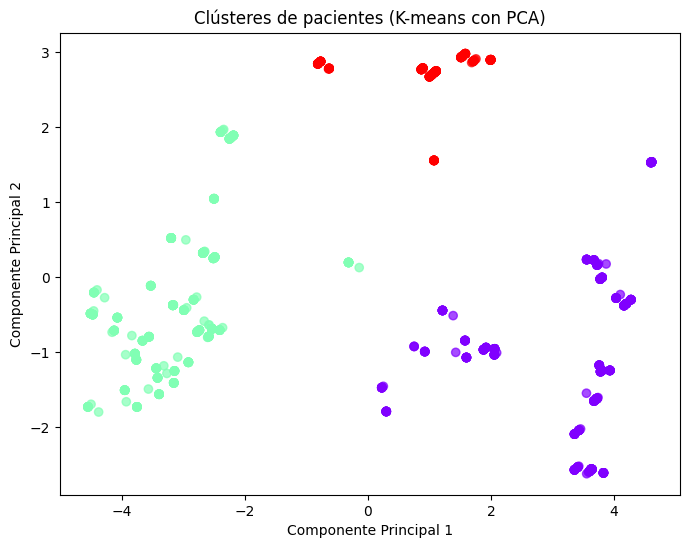
\includegraphics[scale = 0.6]{Enrique/Imagenes/k-means-2d.png}
    \caption{k-means con PCA en 2D}
\end{figure}

En la gráfica de \textit{k-means} con \textit{PCA} en 2D podemos apreciar que se observan significativamente menos de 1,000 puntos, esto se debe a la pérdida y distorsión de datos que se sufrió al aplicar \textit{PCA}, pues como se aprecia en la gráfica de su varianza, solo se recupera el 51.32\%. 

\begin{figure}[H]
    \centering
    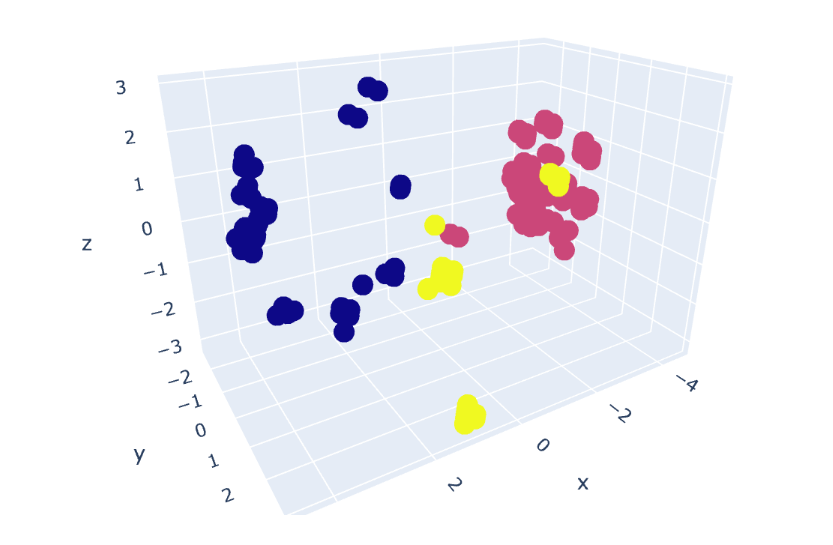
\includegraphics[scale = 0.6]{Enrique/Imagenes/k-means-3d.png}
    \caption{k-means con PCA en 3D}
\end{figure}

En la gráfica de \textit{k-means} con \textit{PCA} en 3D parecieria que el número de observaciones aumentes, lo cuál tiene sentido ya que la varianza total aumentó a 60.90\% al realizar \textit{PCA} para 3 componentes, sin embargo seguimos teniendo una pérdida de datos bastante significativa. 

\subsubsection{Evaluación del modelo}

A continuación mostramos la matriz de confusión que obtuvimos con respecto al agrupamiento de \textit{k-means}

\begin{figure}[H]
    \centering
    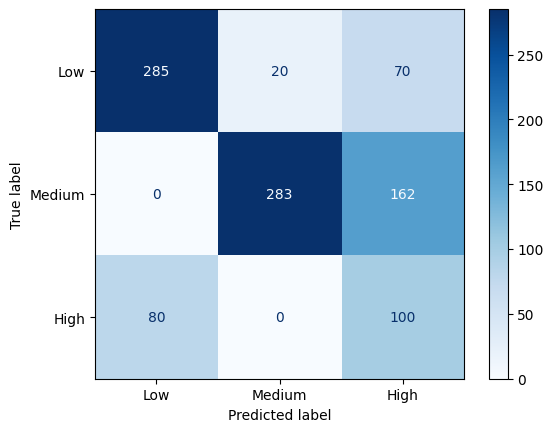
\includegraphics[scale = 0.6]{Enrique/Imagenes/matriz_confusion_k-means.png}
    \caption{Matriz de confusión del modelo \textit{k-means}}
    \label{fig:enter-label}
\end{figure}

De la cual podemos se obtiene el siguiente reporte:

\begin{table}[H]
    \centering
    \begin{tabular}{l c c c c}
        & precision & recall & f1-score & support \\
        Low & 0.78 & 0.76 & 0.77 & 375 \\
        Medium & 0.93 & 0.64 & 0.76 & 445 \\
        High & 0.30 & 0.56 & 0.39 & 180 \\
        accuracy & & & 0.67 & 1000 \\
        macro avg & 0.67 & 0.65 & 0.64 & 1000 \\
        weighted avg & 0.76 & 0.67 & 0.70 & 1000
    \end{tabular}
    \caption{Reporte de clasificación de \textit{k-means} }
\end{table}
  
\subsubsection{Evaluación de DBSCAN}

Pare el método \textit{DBSCAN} obtuvimos la siguiente matriz de confusión

\begin{figure}[H]
    \centering
    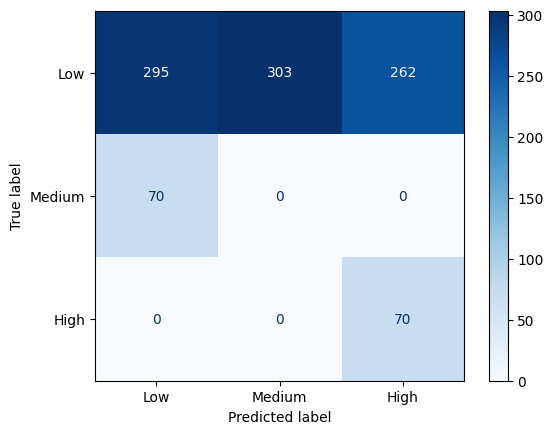
\includegraphics[scale = 0.6]{Enrique/Imagenes/matriz_confusion_DBSCAN.png}
    \caption{Matriz de confusión para \textit{DBSCAN}}
\end{figure}

\begin{table}[H]
    \centering
    \begin{tabular}{l c c c c}
        & precision & recall & f1-score & support \\
        Low    & 0.81 & 0.34 & 0.48 & 860 \\
        Medium & 0.00 & 0.00 & 0.00 & 70 \\
        High   & 0.21 & 1.00 & 0.35 & 70 \\
        accuracy & & & 0.36 & 1000 \\
        macro avg & 0.34 & 0.45 & 0.28 & 1000 \\
        weighted avg & 0.71 & 0.36 & 0.44 & 1000
    \end{tabular}
    \caption{Reporte de clasificación de \textit{DBSCAN} }
\end{table}
               





